\documentclass[utf8,hauptseminar]{zihpub}

\usepackage{datetime}
\usepackage{etoolbox}
\usepackage[acronyms]{glossaries}
\usepackage{listings}
\usepackage[section]{minted}
\usepackage{tcolorbox}
%\usepackage[dvipsnames]{xcolor}

\newdateformat{titledate}{\ordinalnum{\THEDAY} \monthname[\themonth], \THEYEAR}

\BeforeBeginEnvironment{minted}{\begin{tcolorbox}}
\AfterEndEnvironment{minted}{\end{tcolorbox}}

\newcommand{\lstfont}[1]{\color{#1}\small\ttfamily}

%\lstset{language=[11]C++,
%		showstringspaces=false,
%		basicstyle=\lstfont{black},
%		keywordstyle=\lstfont{magenta},
%		stringstyle=\lstfont{orange},
%		emph={cudaMalloc, cudaFree, __global__},
%		emphstyle=\lstfont{magenta},
%		breaklines=true}

\author{Jan Stephan}
\title{Innovations in C++11, 14 and 17 in the Context of Performance Analysis of HPC Applications}
\matno{3755136}
\betreuer{Ronny Brendel}

\newacronym{raii}{RAII}{Resource Acquisition is Initialization}
\newacronym{stl}{STL}{Standard Template Library}

\makeglossaries

\begin{document}

\section{Introduction}

With the release of the C++11 standard in 2011 the C++ community was introduced to several new language and library features~\cite{cpp11std}. Together with a new programming philosophy (see Section~\ref{subs:intro_philosophy}) these changes were so extensive that the original creator of the C++ programming language, Bjarne Stroustrup, felt like it was a ``new language''~\cite{tcpp}.

In this report some of the new features will be presented, especially those which are relevant in a performance analysis context. Additionally, the performance analysis tools Score-P and Vampir will be evaluated with regard to these new changes.

\subsection{C++11 and C++14}

\subsection{The Modern C++ Philosophy}\label{subs:intro_philosophy}

\section{Example: CUDA Vector Addition}

To illustrate some of the features introduced in C++11 and C++14 we will implement a simple vector addition with the CUDA toolkit.

\subsection{The Kernel}

A kernel which implements a vector addition could look like the following:

\begin{lstlisting}
__global__ void vector_add(const int* a, const int* b, int* c, size_t size)
{
    int i = threadIdx.x + blockIdx.x * blockDim.x;
    if(i < size)
        c[i] = a[i] + b[i];
}
\end{lstlisting}

As of CUDA 7 the toolkit supports a subset of the features introduced in C++11. We will use this subset to change the kernel as follows:

\begin{lstlisting}
__global__ void vector_add(const std::int32_t* a, const std::int32_t* b, std::int32_t* c, std::size_t size)
{
    auto i = threadIdx.x + blockIdx.x * blockDim.x;
    if(i < size)
        c[i] = a[i] + b[i];
}
\end{lstlisting}

\subsubsection{Fixed Width Integer Types}

The first notable change is the migration from plain \texttt{int} to \texttt{std::int32\_t}. The latter is called a \textit{fixed width integer type} and was introduced with the C++11 standard which in turn based this inclusion on the C99 standard. These types (ranging from 8bit to 64bit types, both signed and unsigned), along with counterparts optimized for size and performance, can be found in \texttt{<cstdint>}.

\subsubsection{The \texttt{auto} Keyword}

In C++11 the already existing keyword \texttt{auto} changed its meaning. In old standards it denoted the storage class of a variable:

\begin{lstlisting}
void f()
{
    auto int i; // automatic storage class, lives until the end of the scope
    static int j; // static storage class, permanent duration
}
\end{lstlisting}

As the usage of this keyword was largely redundant its meaning was changed in C++11 to deduce the type of an expression:

\begin{lstlisting}
auto i = 0; // i is deduced to be an int
auto f1 = float(0); // committing to a specific type
auto f2 = 0.f; // committing to a specific type, shorthand
auto two = std::sqrt(4); // type deduction from return value
\end{lstlisting}

\texttt{auto} can also be used in combination with functions:

\begin{lstlisting}
auto f() -> void;

template <class T, class U>
auto add(T a, U b) -> decltype(a + b)
{
    return a + b;
}
\end{lstlisting}

The \textit{trailing return type} syntax is especially useful when used with templates, as the second example shows. With C++14 the return type is no longer needed (as long as the function body is visible to the compiler):

\begin{lstlisting}
template <class T, class U>
auto add(T a, U b)
{
    // add's return value deduced to be decltype(a + b)
    return a + b;
}
\end{lstlisting}

According to Herb Sutter\cite{sutteraaa} one should follow an \textit{Almost Always Auto (AAA)} pattern.

\subsection{Host Memory Management}



\subsubsection{The \texttt{constexpr} Keyword}
\subsubsection{Smart Pointers}


\subsection{Device Memory Management}

\subsubsection{The \texttt{using} Keyword}

\subsection{Launching the Kernel}

\subsubsection{Variadic Templates}

\subsection{Overview}
\subsection{Producer/Consumer Queue}\label{modern:queue}

A simple producer/consumer queue is implemented in the following sections to showcase the modern C++ concurrency features.

\subsubsection{C++11 Thread Support}\label{modern:queue:support}

Before the new C++ standard was published in 2011 there was no standardised way to create and manage threads in a platform independent manner. The programmer had to resort to mechanisms specific to the targetted operating system, e.g. Pthreads or Win32 threads, or third-party libraries like Qt. Furthermore these mechanisms are not idiomatic as they are usually plain C interfaces. This means there was no native support for \gls{raii}, making wrappers around these interfaces necessary. Additionally, there was no platform-independent support for atomic operations.

With the adoption of C++11 the situation changed: the new standard introduced a thread support library~\cite{cpp11std}(§30) and an atomic operations library~\cite{cpp11std}(§29). Both will be briefly introduced in the following sections.

\subsubsection{High-level Thread Creation}\label{modern:queue:futures}

The easiest way to spawn concurrent threads in C++11 is to not do it by oneself. Instead, the highest-level approach C++11 offers is a call to \texttt{std::async}~\cite{cpp11std}(§30.6.8), leaving thread creation and management to the library. The result (if any) of the concurrent computation can be collected later by using the \texttt{std::future} construct. With this approach a program relying on a shared queue (which will be implemented in the Sections \ref{modern:queue:mutex} and \ref{modern:queue:atomics}) can be implemented as follows:

\begin{minted}[fontsize=\small]{c++}
#include <future>
using namespace std;

auto main() -> int {
    auto q = queue{};
    // async returns a future which will contain the result
    auto f1 = async(launch::async, [&q](){ q.push(create_object()); });
    auto f2 = async(launch::async, [&q](){ return q.pop(); });
 
    // f1 does not return anything
    f1.get();

    // f2 returns an object
    auto o = f2.get();

    return 0;
}
\end{minted}

\paragraph{std::async}

Note the explicit specification of \texttt{std::launch::async}. By default, one passes a function and an arbitrary number of arguments to \texttt{std::async}. This is equivalent to the following call:

\begin{minted}[fontsize=\small]{c++}
using namespace std;
auto f = async(launch::async | launch::deferred, func, params...);
\end{minted}

\begin{itemize}
\item \texttt{std::launch::async} explicitly tells the library to run the specified function in a separate thread. If \texttt{std::future::get} or \texttt{std::future::wait} are called before the task is completed, the calling thread is blocked until the result becomes ready.
\item \texttt{std::launch::deferred} is the opposite: The function is to be executed on the first call to either \texttt{std::future::get} or \texttt{std::future::wait} and in the same thread as its caller.
\item \texttt{std::launch::async | std::launch::deferred} shows implementation-defined behaviour, i.e. may either spawn a new thread or execute in the same thread as the caller.
\end{itemize}

\noindent In either case the computation's result is stored in the associated \texttt{std::future} and can be accessed by a call to \texttt{std::future::get}.

\paragraph{Lambda functions}

The second parameter to \texttt{std::async} in the example is called a lambda function. This language extension~\cite{cpp11std}(§5.1.2) provides an easy way to create simple functions in-place. It has the following syntax:

\begin{verbatim}
[capture clause](parameters){ body }
\end{verbatim}

\noindent The \textit{capture clause} tells the compiler how to make names outside of the lambda's body visible on the inside. An empty clause (\texttt{[]}) prevents any access to names outside of the lambda. A reference clause (\texttt{[\&]}) captures all names by reference, a copy clause (\texttt{[=]}) copies them. These operations are also applicable to single names: \texttt{[\&foo]} captures only \texttt{foo} by reference, \texttt{[=bar]} copies only \texttt{bar}. The latter is equivalent to \texttt{[bar]}. Additionally, these operations are combinable: \texttt{[\&foo, bar]} captures \texttt{foo} and copies \texttt{bar}.

The parameters and the body work mostly like those of a normal function, except that the parameters can be generic (declared as \texttt{auto}) as well since C++14~\cite{cpp14std}(§5.1.2).

\subsubsection{Low-level Thread Creation}\label{modern:queue:threads}

A manual approach to thread management is offered by \texttt{std::thread}~\cite{cpp11std}(§30.3.1). It works in a very similar way to the Pthread library:

\begin{minted}[fontsize=\small]{c++}
#include <thread>

auto main() -> int {
    auto q = queue{};
    auto obj = object{};
    auto p = std::thread([&q](){ q.push(create_object()); });
    auto c = std::thread([&q, &obj](){ obj = q.pop(); });
    
    p.join();
    c.join();
    
    return 0;
}
\end{minted}

\noindent In contrast to \texttt{std::async} there is no direct way to obtain the result of the computation; instead it is the programmer's responsibility to obtain the result in a way of his choosing, e.g. by passing an empty object by reference or by handcrafting a solution around \texttt{std::future} and its companion \texttt{std::promise}.

\subsubsection{High-level Synchronisation}\label{modern:queue:mutex}

Whenever multiple threads are accessing the same data synchronisation becomes an important issue. For this purpose the C++11 standard includes synchronisation constructs, namely \texttt{std::mutex}, its derivates and locking mechanisms~\cite{cpp11std}(§30.4) as well as \texttt{std::condition\_variable}~\cite{cpp11std}(§30.5). The latter offers a more fine-grained control over blocking or unblocking threads and is always bound to a \texttt{std::mutex}.

A shared queue utilizing \texttt{std::mutex} and \texttt{std::condition\_variable} could be implemented as follows:

\begin{minted}[fontsize=\small]{c++}
#include <condition_variable>
#include <mutex>
#include <queue>

template <class T>
class queue {
    public:
        auto push(T t) -> void {
            auto lock = std::unique_lock<std::mutex>{m_};
            
            queue_.push(std::move(t));
            cv_.notify_one();
        }
        
        auto pop() -> T {
            auto lock = std::unique_lock<std::mutex>{m_};
            while(queue_.empty())
                cv_.wait(lock);
                
            auto ret = std::move(queue_.front());
            queue_.pop();
            
            return ret;
        }
        
    private:
        std::condition_variable cv_;
        std::mutex m_;
        std::queue<T> queue_;
};
\end{minted}

\noindent Once an object is pushed to the \texttt{queue}, the \texttt{std::mutex} is locked. Instead of calling \texttt{std::mutex}'s member functions \texttt{lock} and \texttt{unlock} directly, \gls{raii} is utilized by constructing a \texttt{std::unique\_lock} object. The object is then pushed to the internal \texttt{std::queue}. Afterwards, another thread that is waiting to access the (previously empty) \texttt{queue} is notified.

Popping an object works similarly: first, the lock is obtained. Then, if the internal \texttt{std::queue} happens to be empty, the lock is released temporarily until another thread calls \texttt{notify\_one}, a member function of \texttt{std::condition\_variable}. Afterwards the first object in the queue is obtained and returned to the caller.

\subsubsection{Low-level Synchronisation}\label{modern:queue:atomics}

Besides the high-level constructs presented in Section \ref{modern:queue:mutex}, C++11 also introduced atomic operations to the standard library. These offer another way to synchronise threads and leave more control (and responsibility) to the programmer. \texttt{std::atomic\_flag} is especially useful for synchronisation constructs and can replace \texttt{std::mutex} in the shared queue implemented above:

\begin{minted}[fontsize=\small]{c++}
#include <atomic>
#include <thread>
#include <queue>

template <class T>
class queue {
    public:
        auto push(T t) -> void {
            while(lock_.test_and_set())
                std::this_thread::yield();
                
            queue_.push(std::move(t));
            lock_.clear();
        }
        
        auto pop() -> T {
            while(queue_.empty())
                std::this_thread::yield();
                
            while(lock_.test_and_set())
                std::this_thread::yield();
                
            auto ret = std::move(queue_.front());
            queue_.pop();
            
            lock_.clear();
            return ret;
        }
        
        private:
            std::atomic_flag lock_ = ATOMIC_FLAG_INIT;
            std::queue<T> queue_;
};
\end{minted}

\noindent The disadvantage of this approach is that it is not intuitive. \texttt{std::atomic\_flag::test\_and\_set} atomically sets the flag to \texttt{true} and returns the previous value. In this context \texttt{true} means ``locked''. The \texttt{while} loop will only break if another thread has cleared the flag, i.e. set it to \texttt{false}. In this case the flag is set to \texttt{true} by the current thread (thus blocking other threads), the current thread performs its work and then clears the flag (thus unblocking other threads).

From an outside perspective both implemented queues behave the same: There can be only one thread accessing the data, all  other threads have to wait for it to complete its work.
%\section{Improving Maintainability: Implementing the Blowfish Algorithm}

\subsection{The Blowfish Algorithm}
% ERSTEN SATZ UMFORMULIEREN
A technical description of the Blowfish algorithm is outside of this paper's scope; the inclined reader may refer to \cite{blowfish} for further information about its theoretical foundation. In the following sections we will port OpenSSL's basic Blowfish algorithm (ECB), as implemented by OpenSSL 1.0.2h. %REFERENZ!!!

\subsection{Maintainability Improvements}

As noted before (see Section \ref{subs:intro_philosophy}) the C++ standard library offers a variety of abstractions that reduce the amount of code needed for specific intents. As Garcia and Stroustrup noted the usage of abstraction based refactoring "improve[s] the performance, flexibility, and maintainability of a large class of programs"~\cite{impperf}.

We can utilize these techniques to refactor OpenSSL's Blowfish encryption algorithm into a modern C++ implementation which offers similar performance while reducing the code size.

\subsection{Porting OpenSSL's Implementation}

\subsubsection{Interface}\label{subsub:bf_interface}

OpenSSL offers the following interface for a basic ECB encryption:

\begin{lstlisting}[language=C]
#define BF_LONG unsigned int // has to be at least 32 bits wide
#define BF_ROUNDS 16

typedef struct bf_key_st {
    BF_LONG P[BF_ROUNDS + 2];
    BF_LONG S[4 * 256];
} BF_KEY;

void BF_set_key(BF_KEY *key, int len, const unsigned char *data);
void BF_encrypt(BF_LONG *data, const BF_KEY *key);
void BF_decrypt(BF_LONG *data, const BF_KEY *key);

void BF_ecb_encrypt(const unsigned char *in, unsigned char *out, const BF_KEY *key, int enc);
\end{lstlisting}

This C interface can be changed to the following to remove the need for pointers, function prefixes and the preprocessor:

\begin{lstlisting}[language=C++]
// use namespaces to prevent pollution of the global namespace
namespace bf
{
    // use real compile time constants
    constexpr auto rounds = 16;
    
    // use portable integer types and std::array instead of plain arrays
    struct key {
        array<uint32_t, rounds + 2> p;
        array<uint32_t, 4 * 256> s;
    };
    
    // use strongly-typed enums instead of integers for function selection
    enum class enc {
        encrypt,
        decrypt
    };
    
    // use std::vector for arbitrary lengths
    auto set_key(const vector<uint8_t>& data) -> key;
    // use std::array for compile-time lengths and take key by reference
    auto encrypt(array<uint32_t, 2>& data, const key& k) -> void;
    auto decrypt(array<uint32_t, 2>& data, const key& k) -> void;
    
    auto ecb_encrypt(const vector<uint8_t>& in, vector<uint8_t>& out, const key& k, enc e) -> void;
}
\end{lstlisting}

\subsubsection{Implementation}

In this section we will cover the actual porting of the algorithm's implementation; however, an in-depth explanation is beyond the scope of this document. A full implementation is provided in Appendix \ref{app:blowfish}.

\paragraph{Key Creation}

At the program startup OpenSSL sets up a \texttt{static const BF\_KEY} variable whose fields are initialized with values derived from the hexadecimal digits of pi. When first creating a \texttt{BF\_KEY} OpenSSL will \texttt{memcpy} this variable to the pointer passed to the function:

\begin{lstlisting}[language=C]
static const BF_KEY bf_init = { /* ... */ };

void BF_set_key(BF_KEY *key, int len, const unsigned char *data)
{
    memcpy(key, &bf_init, sizeof(BF_KEY));
    // ...
}
\end{lstlisting}

This \texttt{memcpy} would not be necessary even in plain C; a simple assignment expresses intent in a better way and enables more optimizations by the compiler:

\begin{lstlisting}[language=C]
static const BF_KEY bf_init = { /* ... */};

void BF_set_key(BF_KEY *key, int len, const unsigned char *data)
{
    *key = bf_init;
    // ...
}
\end{lstlisting}

As \texttt{bf\_init}'s values are hard-coded we can easily declare them compile time constants. Since these values are only needed once they also do not need to live outside of the source file which is why we can easily put them into an anonymous namespace to prevent any external dependencies on them\footnote{Unnamed (anonymous) namespaces have the same effect as the \texttt{static} keyword on variables and functions. However, they can also be used for types which makes them superior to \texttt{static}; it is impossible to declare a \texttt{static struct}, for example.}. After adjusting the code according to the C++ interface mentioned in Section \ref{subsub:bf_interface} the result looks similar to the following excerpt:

\begin{lstlisting}[language=C++]
namespace bf
{
    namespace
    {
        constexpr auto init = key { /* ... */ };
    }
    
    auto set_key(const vector<uint8_t>& data) -> key
    {
        auto k = init;
        // ...
    }
}
\end{lstlisting}

The rest of the code remains mostly unchanged as it largely consists of binary operations.

\paragraph{Encryption and Decryption}

OpenSSL's routines for encryption and decryption of a 64 bit array (containing two 32 bit unsigned integers) call the same macro a 

\subsubsection{Comparison}
\section{Support in Score-P and Vampir}

In the following sections the level of support for modern C++ by Score-P and Vampir will be discussed. This is achieved by implementing several small example programs that make use of these features. The source code of these examples can be found in Appendix \ref{app:scorep}. The code is compiled with gcc 6.2.1, using the compiler plugin from Score-P 3.0. The results are examined using Vampir 9.0.

\subsection{Concurrency}\label{scorep:conc}

In this section the various concurrency constructs introduced in C++11 will be discussed.

\subsubsection{\texttt{std::async}}\label{scorep:conc_async}

As mentioned in Section \ref{queue} \texttt{std::async} is a high-level construct to asynchronously run tasks. The underlying management of this asynchronous is not exposed to the library user; instead, it is guaranteed that the result is returned upon a call to \texttt{future::get} (\texttt{std::async} returns a \texttt{std::future}). This may lead to blocking on the caller's side if the asynchronous task has not been completed yet. This potential bottleneck makes any application using \texttt{std::async} a natural target for profiling, even more so as its default behaviour with regard to thread spawning is implementation specific.

There are three test cases in this document: One for the default behaviour (Appendix \ref{app:scorep_conc_async_default}), another for explicit asynchronous evaluation (Appendix \ref{app:scorep_conc_async_async}) and a third for explicit lazy evaluation (Appendix \ref{app:scorep_conc_async_lazy}).

The first two test cases fail with the following error message:

\begin{verbatim}
$ SCOREP_ENABLE_TRACING=1 ./future_default                                      
[Score-P] src/measurement/thread/create_wait/scorep_thread_create_wait
          _pthread.c:84: Fatal: Bug 'tpd == 0': Invalid Pthread thread
          specific data object. Please ensure that all pthread_create
          calls are instrumented.
[Score-P] Please report this to support@score-p.org. Thank you.
[Score-P] Try also to preserve any generated core dumps.
[Score-P] src/measurement/thread/create_wait/scorep_thread_create_wait
          _pthread.c:84: Fatal: Bug 'tpd == 0': Invalid Pthread thread
          specific data object. Please ensure that all pthread_create
          calls are instrumented.[1]    8405 abort (core dumped)
\end{verbatim}

Unfortunately, imitating \texttt{std::async}'s behaviour with Pthreads for the sake of this document is impossible as the thread management behind the call is implementation-defined: the library may spawn simple Pthreads internally, rely on a thread pool or do something entirely different.

The lazy evaluation test case executes successfully; however, because the code in question is not executed in a separate thread the inspection of Score-P's trace file shows nothing noteworthy (see Figures \ref{scorep:conc_async_lazy_timeline} and \ref{scorep:conc_async_lazy_summary}).

\begin{figure}[htbp]
	\begin{center}
		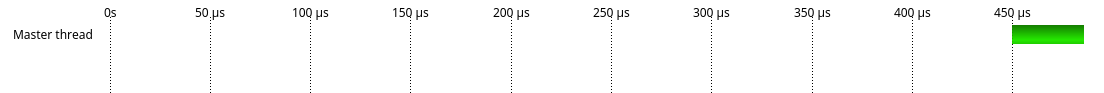
\includegraphics[width=0.9\textwidth]{img/scorep_async_lazy_timeline.png}
		\caption{Master timeline for \texttt{std::async} with lazy evaluation}
		\label{scorep:conc_async_lazy_timeline}
	\end{center}
\end{figure}

\begin{figure}[htbp]
	\begin{center}
		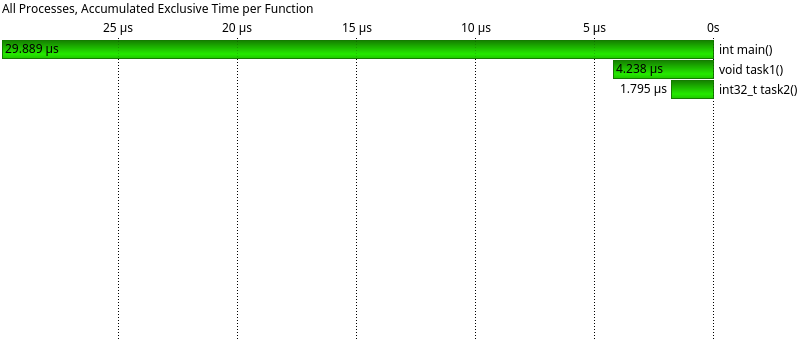
\includegraphics[width=0.9\textwidth]{img/scorep_async_lazy_summary.png}
		\caption{Function summary for \texttt{std::async} with lazy evaluation}
		\label{scorep:conc_async_lazy_summary}
	\end{center}
\end{figure}

\subsubsection{\texttt{std::thread}}\label{scorep:conc_thread}

When compared to \texttt{std::async} \texttt{std::thread} follows a much more ``low level'' approach as thread execution is now entirely in the hands of the user. Naturally C++11 threads are profiling targets as well as they build the very foundation of modern C++ style concurrent programming.

There is are two test cases for \texttt{std::thread}: the first spawns a thread and joins it afterwards (Appendix \ref{app:conc_thread_join}), the second spawns a thread and detaches it, making it unjoinable (Appendix \ref{app:conc_thread_detach}).

Both test cases fail to execute and produce the same error message already known from Section \ref{scorep:conc_async}. Because \texttt{std::thread} simply wraps a Pthread (at least in libstdc++) its behaviour can be emulated (see Figures \ref{scorep:conc_pthread_join_timeline} and \ref{scorep:conc_pthread_join_summary} and Figures \ref{scorep:conc_pthread_detach_timeline} and \ref{scorep:conc_pthread_detach_summary}, respectively).

\begin{figure}[htbp]
	\begin{center}
		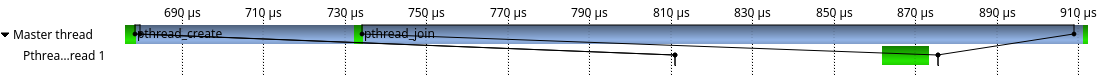
\includegraphics[width=0.9\textwidth]{img/scorep_pthread_join_timeline.png}
		\caption{Emulated master timeline for a joined \texttt{std::thread}}
		\label{scorep:conc_pthread_join_timeline}
	\end{center}
\end{figure}

\begin{figure}[htbp]
	\begin{center}
		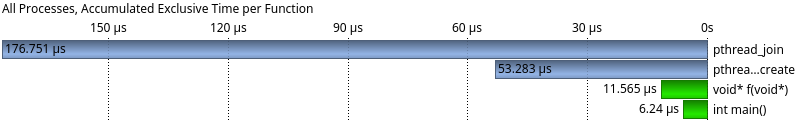
\includegraphics[width=0.9\textwidth]{img/scorep_pthread_join_summary.png}
		\caption{Emulated function summary for a joined \texttt{std::thread}}
		\label{scorep:conc_pthread_join_summary}
	\end{center}
\end{figure}

\begin{figure}[htbp]
	\begin{center}
		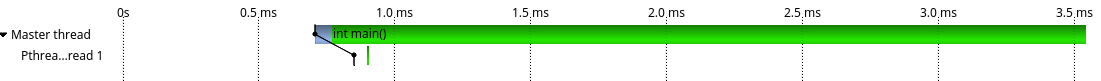
\includegraphics[width=0.9\textwidth]{img/scorep_pthread_detach_timeline.png}
		\caption{Emulated master timeline for a detached \texttt{std::thread}}
		\label{scorep:conc_pthread_detach_timeline}
	\end{center}
\end{figure}

\begin{figure}[htbp]
	\begin{center}
		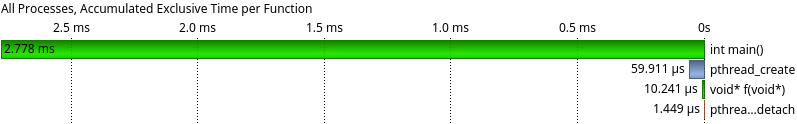
\includegraphics[width=0.9\textwidth]{img/scorep_pthread_detach_summary.png}
		\caption{Emulated function summary for a detached \texttt{std::thread}}
		\label{scorep:conc_pthread_detach_summary}
	\end{center}
\end{figure}

\subsubsection{Summary}

At the time of writing, Score-P's support for C++11 multithreading is nonexistent as the error messages from Section \ref{scorep:conc_async} and Section \ref{scorep:conc_thread} show. The likely cause for these errors lies in the internals of the GNU C++ compiler's standard library as the threading support library is compiled into the shared library object. Score-P is unable to instrument this already compiled code and crashes upon execution once it encounters an unknown thread.

The solution for this problem would be a more graceful handling of ``unknown threads'': Instead of crashing Score-P should simply register them on the fly.

\subsection{Synchronization}

With the introduction of the thread support library synchronization primitives were added to the standard library as well. As such primitives are able to block thread execution profiling their behaviour is especially interesting in a HPC context. In this section the mutual exclusion constructs (\texttt{std::mutex}) and condition variables (\texttt{std::condition\_variable}) are evaluated. Due to the problems shown in Section \ref{scorep:conc} the spawned threads in the testcases are classic Pthreads.

\subsubsection{\texttt{std::mutex}}\label{scorep:sync_mutex}

\texttt{std::mutex} and its more specialized siblings \texttt{std::timed\_mutex}, \texttt{std::recursive\_mutex} and \texttt{std::recursive\_timed\_mutex} provide simple mechanisms for mutual exclusion between threads. Like similar primitives these constructs provide mechanisms for locking and unlocking. However, directly accessing these mechanisms is not exception-safe which is why they are usually managed by \texttt{std::unique\_lock} or \texttt{std::lock\_guard}. Relying on \gls{raii} these primitives will automatically unlock the managed \texttt{std::mutex} once they go out of scope.

The test case (see Appendix \ref{app:scorep_sync_mutex}) utilizes them as well for synchronization between two threads instead of locking the \texttt{std::mutex} manually. Upon execution the test case itself works as expected: Pthreads are spawned and \texttt{std::mutex} blocks one of them while being locked by the other.

Score-P on the other hand is not able to fully parse the instruction flow correctly: instead of instrumenting the calls to the standard library facilites it detects and instruments the underlying  Pthread mechanisms utilized by the library implementation (see Figures \ref{scorep:sync_pthread_mutex_timeline} and \ref{scorep:sync_pthread_mutex_summary}). This can be explained by the compiler's aggressive inlining of the \gls{stl} functions which prevents Score-P from instrumenting the actual function call.

\begin{figure}[htbp]
	\begin{center}
		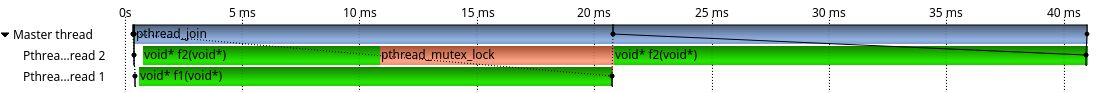
\includegraphics[width=0.9\textwidth]{img/scorep_pthread_mutex_timeline.png}
		\caption{Master timeline for thread synchronization with \texttt{std::mutex}}
		\label{scorep:sync_pthread_mutex_timeline}
	\end{center}
\end{figure}

\begin{figure}[htbp]
	\begin{center}
		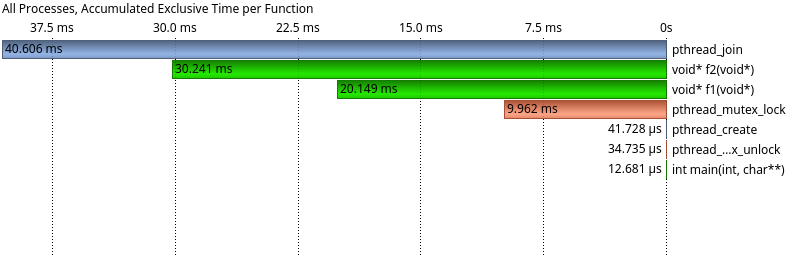
\includegraphics[width=0.9\textwidth]{img/scorep_pthread_mutex_summary.png}
		\caption{Function summary for thread synchronization with \texttt{std::mutex}}
		\label{scorep:sync_pthread_mutex_summary}
	\end{center}
\end{figure}

\subsubsection{\texttt{std::condition\_variable}}

The other synchronization primitive added to the standard library with C++11 is \texttt{std::condition\_variable} which allows threads to communicate with each other. A \texttt{std::condition\_variable} is always associated with a \texttt{std::mutex} but offers more fine-grained control via its notification mechanisms -- a thread can either wake up one other waiting thread or all of them.

The test case (see Appendix \ref{app:scorep_sync_cv}) spawns four Pthreads, of which three are waiting for the fourth to signal them. Once they receive the notification they execute their instructions in parallel.

Like the simpler \texttt{std::mutex} test case (see Section \ref{scorep:sync_mutex}) this program executes successfully and suffers from the same problems with inlining (see Figures \ref{scorep:sync_pthread_cv_timeline} and \ref{scorep:sync_pthread_cv_summary}).

\begin{figure}[htbp]
	\begin{center}
		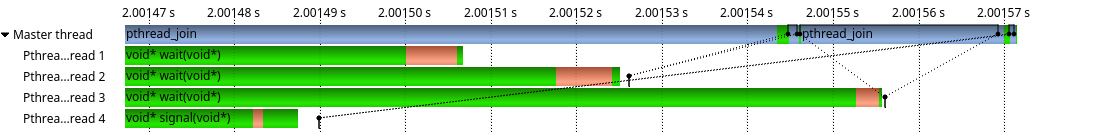
\includegraphics[width=0.9\textwidth]{img/scorep_pthread_cv_timeline.png}
		\caption{Master timeline for thread synchronization with \texttt{std::condition\_variable}}
		\label{scorep:sync_pthread_cv_timeline}
	\end{center}
\end{figure}

\begin{figure}[htbp]
	\begin{center}
		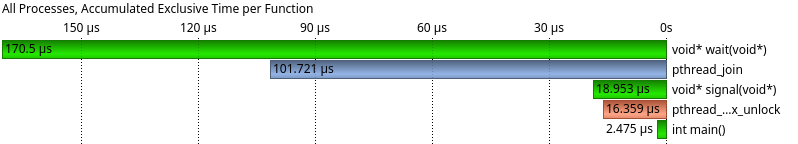
\includegraphics[width=0.9\textwidth]{img/scorep_pthread_cv_summary.png}
		\caption{Function summary for thread synchronization with \texttt{std::condition\_variable}}
		\label{scorep:sync_pthread_cv_summary}
	\end{center}
\end{figure}

\subsubsection{Summary}

While Score-P's support for synchronization primitives is better than its support for C++11 threads it is not perfect. Due to aggressive compiler inlining the \gls{stl} functions are optimized away before Score-P can instrument them. In order to change this Score-P would need a mechanism to instrument the \gls{stl}'s interface without automatically instrumenting all the implementation details behind the interface because those are likely to be inlined as well.

\subsection{File I/O}

While file I/O is not a new concept and has not changed with C++11 its performance penalties are still an important issue to consider in an HPC context. In this section file I/O using binary file streams, text file streams and (for comparison) the C API will be evaluated.

\subsubsection{Binary I/O}\label{scorep:binary_fstream}

The first test case (see Appendix \ref{app:scorep_binary_fstream}) generates a \texttt{std::vector} with random integer values and writes them to a file. The file itself is created and modified by a \texttt{std::ofstream} opened in binary mode. It is then closed and opened again in binary mode by a \texttt{std::ifstream} which then proceeds to read its contents into another \texttt{std::vector}.

As the Figures \ref{scorep:binary_fstream_timeline} and \ref{scorep:binary_fstream_summary} show all of the aforementioned  are ignored entirely by Score-P's instrumentation.

\begin{figure}[htbp]
	\begin{center}
		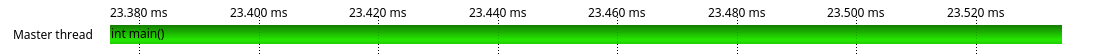
\includegraphics[width=0.9\textwidth]{img/scorep_binary_fstream_timeline.png}
		\caption{Master timeline for file operations using \texttt{std::fstream} in binary mode}
		\label{scorep:binary_fstream_timeline}
	\end{center}
\end{figure}

\begin{figure}[htbp]
	\begin{center}
		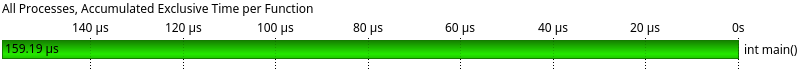
\includegraphics[width=0.9\textwidth]{img/scorep_binary_fstream_summary.png}
		\caption{Function summary for file operations using \texttt{std::fstream} in binary mode}
		\label{scorep:binary_fstream_summary}
	\end{center}
\end{figure}

\subsubsection{Text I/O}

The second test case (see Appendix \ref{app:scorep_text_fstream}) uses a \texttt{std::ofstream} in text mode to output a text to a file. This file is then closed and reopened by a \texttt{std::ifstream} in text mode, the contents are printed to \texttt{stdout}.

Again, Score-P fails to instrument any of the instructions (Figures \ref{scorep:text_fstream_timeline} and \ref{scorep:text_fstream_summary}).

\begin{figure}[htbp]
	\begin{center}
		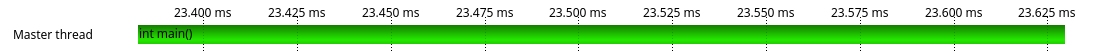
\includegraphics[width=0.9\textwidth]{img/scorep_text_fstream_timeline.png}
		\caption{Master timeline for file operations using \texttt{std::fstream} in text mode}
		\label{scorep:text_fstream_timeline}
	\end{center}
\end{figure}

\begin{figure}[htbp]
	\begin{center}
		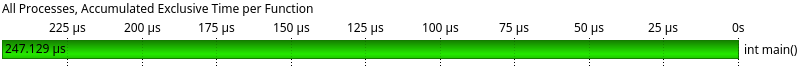
\includegraphics[width=0.9\textwidth]{img/scorep_text_fstream_summary.png}
		\caption{Function summary for file operations using \texttt{std::fstream} in text mode}
		\label{scorep:text_fstream_summary}
	\end{center}
\end{figure}

\subsubsection{C-style I/O}

The results of the previous sections may lead to the conclusion that the file operations are inlined by the compiler and thus not visible to Score-P. The third test case implements the functionality from Section \ref{scorep:binary_fstream} using the API inherited from the C standard library (see Appendix \ref{app:scorep_c_io}).

Figures \ref{scorep:c_io_timeline} and \ref{scorep:c_io_summary} show that the issue is not related to inlining. 

\begin{figure}[htbp]
	\begin{center}
		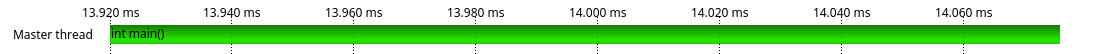
\includegraphics[width=0.9\textwidth]{img/scorep_c_io_timeline.png}
		\caption{Master timeline for file operations using the C standard library API}
		\label{scorep:c_io_timeline}
	\end{center}
\end{figure}

\begin{figure}[htbp]
	\begin{center}
		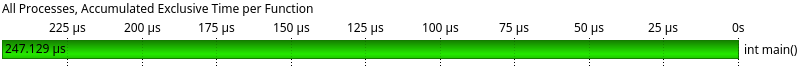
\includegraphics[width=0.9\textwidth]{img/scorep_text_fstream_summary.png}
		\caption{Function summary for file operations using the C standard library API}
		\label{scorep:c_io_summary}
	\end{center}
\end{figure}

\subsubsection{Summary}

At the time of writing Score-P does not support the instrumentation of file I/O. In order to change this it would need a way to instrument system calls as those are called internally by standard library file operations.

\subsection{Lambdas}

Lambda functions are especially useful when used in conjunction with the functions found in the header file \texttt{<algorithm>}. This naturally makes them a target of interest in a profiling context. Usually they are inlined because of their small code size which renders them invisible for Score-P.

In cases where inlining does not occur Score-P faces two minor naming issues. The first issue can be reproduced by the following code:

\begin{lstlisting}
auto my_lambda = [](int i) { //... };
\end{lstlisting}

If this code does not get inlined for whatever reason\footnote{Unfortunately, this behaviour was not reliably reproducible which is why there is no test case in the appendix. The lambda's symbols are present in the executable but they are still not visible to Score-P.} Score-P will show the following name:

\begin{lstlisting}
main::{lambda(int)#2}::operator()(int) const
\end{lstlisting}

This naming is very unintuitive and does not help the user in quickly identifying hotspots. The situation becomes worse when using an \texttt{auto} parameter, a feature introduced in C++14:

\begin{lstlisting}
auto my_lambda = [](auto i) { // ... };

_ZZ4mainENKUlTE_clIiEEDaS_ // called with "int" parameter
_ZZ4mainENKUlTE_clIdEEDaS_ // called with "double" parameter
\end{lstlisting}

Both issues are not Score-P's fault but originate in GCC's naming and mangling scheme. To work around this, Score-P would need to implement a custom naming mechanism which works around the one imposed by GCC.
\section{Outlook On C++17}\label{cpp17}

This section provides a brief overview for the planned changes of the upcoming C++ standard~\cite{cpp17std}. This revision is likely to be released in 2017.

\subsection{The Standardisation Process}\label{cpp17:standardisation}

When C++11 was released in 2011 thirteen years had passed since the last major C++ standard (C++98) and eight since the last minor standard (C++03). During this time technology has evolved and with it the needed programming models, for example the widespread adoption of multicore CPUs and thus concurrent programming. However, the C++ programming language and its standard library did not reflect this development, forcing developers to rely on third-party libraries such as Boost or Pthreads.

In order to prevent this issue in the future the C++ standard committee was reorganised into several subgroups in 2012, adopting a decentral work process. These subgroups are officially called ``study groups'' and each of them works on evolving a part of the language or the library. As of September 2016 there are 14 study groups~\cite{cpp_committee}, focusing on topics such as low latency, issues with the currently available concurrency features, databases and more.

The overall goal is to publish new standards much more frequently than before. The focus on faster and therefore ``slimmer'' standardisation also has the effect that compiler and standard library developers are able to fully implement the standard much faster~\cite{cpp14_announcement}.

\subsection{\texttt{if}-Statement with Initializer}\label{cpp17:if_init}

The next C++ standard will see a significant change to the core language: \texttt{if}-statements can initialise variables directly. The current way of initialising looks like this:

\begin{minted}[fontsize=\small]{c++}
std::map<int, std::string> m;

auto it = m.find(10);
if(it != m.end()) return it->size();
\end{minted}

\noindent This approach has the disadvantage that \texttt{it} is now visible beyond the \texttt{if}-statement and can not be changed later to e.g. a \texttt{std::vector::iterator}. The upcoming standard enables the developer to change his code to the following~\cite{cpp17std}(§6.4):

\begin{minted}[fontsize=\small]{c++}
std::map<int, std::string> m;

if(auto it = m.find(10); it != m.end()) return it->size();
\end{minted}

\noindent Additionally, \texttt{it} is now only visible inside the scope of the \texttt{if}-statement. This means he can reuse the name later for another purpose.

\subsection{Structured Bindings}\label{cpp17:struct_bind}

Another important change to the core language are \textit{structured bindings}~\cite{cpp17std}(§8.5). These enable the developer to initialise multiple variables at once from a struct:

\begin{minted}[fontsize=\small]{c++}
struct s {
    int x;
    volatile double y;
};

auto f() -> s { // ... }
const auto [x, y] = f();

foo(x); // x is of type const int
bar(y); // y is of type const volatile double
\end{minted}

\noindent In combination with the changes presented in Section \ref{cpp17:if_init} this leads to clean and elegant code:

\begin{minted}[fontsize=\small]{c++}
if(auto [x, y, z] = foo(); x.valid())
    bar(y, z);
\end{minted}

\subsection{Library Extensions}\label{cpp17:lib_ext}

Apart from changes to the core language the upcoming standard will see additions to the standard library as well. Some of those changes are:

\begin{itemize}
\item the switch to the C11 standard as foundation for C++17~\cite{cpp17std}(§1.2)
\item additional mathematical functions (polynomials, beta function, elliptic integrals, etc.)~\cite{cpp17std}(§26.9.5)
\item functions for filesystem interaction ~\cite{cpp17std}(§27.10)
\item new algorithms in the header file \texttt{<algorithm>} (\texttt{sample}, \texttt{reduce}, etc.)~\cite{cpp17std}(§25)
\item parallelisable algorithms (in the header \texttt{<algorithm>})~\cite{cpp17std}(§25)
\end{itemize}

\noindent The last point raises the question how parallelisable algorithms such as \texttt{std::find} are internally implemented (which makes them suitable for specific use cases or not). At the time of writing most of the commonly available standard libraries do not yet support parallel algorithms; however, Microsoft provided an open-source reference implementation~\cite{parallel_stl} to which the inclined reader may refer to learn about the details.
\section{Conclusion}

Modern C++ changed the way of efficient C++ programming tremendously. It leads to a higher abstraction level without a decrease in performance, makes memory management (and thus safety) as well as concurrency a lot easier and offers several other advantages to the HPC community.

The increasing adoption of these changes by developers puts a lot of pressure on performance analysis programs such as Score-P and Vampir. Most of the features offered by C++ and its standard library are already supported or not relevant in a performance analysis context. As this report shows some important features -- especially in the field of concurrency -- are not supported yet. This is an important issue that needs to be addressed quickly if Score-P and Vampir should not become irrelevant in the medium term. Solutions for some of these problems are outlined in this paper; other issues are actively worked on at the time of writing.

Perhaps the most interesting additions (from an HPC perspective) to the standard library will be the parallelisable algorithms from the upcoming standard. Correctly instrumenting and displaying these algorithms at the time of their release would be a great improvement to both Score-P and Vampir and a serious advantage over comparable applications.

The test cases from the appendix, along with their traces and several other example programs, can be found on the author's repository at GitHub: \url{https://github.com/j-stephan/hs16}.
\section{Additional Literature}

Unfortunately, the scope of this document does not permit more than giving a short overview of modern C++. The inclined reader may refer to one or more of the works listed below to follow are more in-depth introduction:

\begin{itemize}
\item Stanley B. Lippmann, Josee Lajoie, Barbara E. Moo: \textit{C++ Primer}, Addison-Wesley, 2012. The intended audience of this book are beginners, both in programming and C++. It follows a high-level approach; for example it starts with containers before explaining dynamic memory allocation.
\item Bjarne Stroustrup: \textit{A Tour of C++}, Addison-Wesley, 2014. This book targets people who have programmed before (not necessarily in C++) and provides them with a broad introduction to the features found in modern C++.
\item Bjarne Stroustrup: \textit{The C++ Programming Language}, Addison-Wesley, 2013. With this work the creator of the C++ programming language published an exhaustive introduction to modern C++, covering the language and its standard library in great detail.
\item Scott Meyers: \textit{Effective Modern C++}, O'Reilly, 2014. Targeting an experienced audience Scott Meyers provides a lot of optimization hints with this work.
\item Anthony Williams: \textit{C++ Concurrency in Action}, Manning, 2012. As the title says this book focuses on modern C++ concurrency mechanisms.
\end{itemize}

Additionally, the following links may help anyone seeking to deepen his knowledge:

\begin{itemize}
\item Bjarne Stroustrup: \textit{C++11 FAQ}, \url{http://www.stroustrup.com/C++11FAQ.html}. This page explains the frequently questioned design decisions of the C++11 standard.
\item Herb Sutter: \textit{Guru of the Week}, \url{https://www.herbsutter.com/gotw/}. In this weekly weblog series Herb Sutter explains C++ features in great depth, usually by providing a puzzle and explaining the solution a week later.
\end{itemize}
\bibliography{bibliography.bib}{}
\begin{appendix}

\section{Basic Blowfish Implementation}\label{app:blowfish}

\subsection{blowfish.h}

\begin{lstlisting}[language=C++]
namespace bf
{
    constexpr auto rounds = 16;
    
    struct key {
        array<uint32_t, rounds + 2> p;
        array<uint32_t, 4 * 256> s;
    };
    
    enum class enc {
        encrypt,
        decrypt
    };
    
    auto set_key(const vector<uint8_t>& data) -> key;
    auto encrypt(array<uint32_t, 2>& data, const key& k) -> void;
    auto decrypt(array<uint32_t, 2>& data, const key& k) -> void;
    
    auto ecb_encrypt(const vector<uint8_t>& in, vector<uint8_t>& out, const key& k, enc e) -> void;
}
\end{lstlisting}

\subsection{ecb.cpp}

\begin{lstlisting}[language=C++]
namespace bf
{
    namespace
    {
        template <class OutputIt>
        inline auto n2l(OutputIt& c, std::uint32_t& l) -> void
        {
            l = static_cast<uint32_t>(*(c++)) << 24L;
            l |= static_cast<uint32_t>(*(c++)) << 16L;
            l |= static_cast<uint32_t>(*(c++)) << 8L;
            l |= static_cast<uint32_t>(*(c++));
        }
        
        template <class InputIt>
        inline auto l2n(std::uint32_t l, InputIt& c) -> void
        {
            *(c++) = static_cast<uint32_t>((l >> 24L) & 0xFF);
            *(c++) = static_cast<uint32_t>((l >> 16L) & 0xFF);
            *(c++) = static_cast<uint32_t>((l >> 8L) & 0xFF);
            *(c++) = static_cast<uint32_t>(l & 0xFF);
        }
    }
    
    auto ecb_encrypt(const vector<uint8_t>& in, vector<uint8_t>& out, const key& k, enc e) -> void
    {
        auto l = uint32_t{};
        auto d = array<uint32_t, 2>{};
        auto in_it = begin(in);

        n2l(in_it, l);
        d.at(0) = l;
        
        n2l(in_it, l);
        d.at(1) = l;
        
        if(e == enc::encrypt)
            encrypt(d, k);
        else
            decrypt(d, k);
            
        auto out_it = begin(out);
        
        l = d.at(0);
        l2n(l, out_it);
        
        l = d.at(1);
        l2n(l, out_it);
        
        l = 0;
        d.at(0) = 0;
        d.at(1) = 0;
    }
\end{lstlisting}

\subsection{encrypt.cpp}

\begin{lstlisting}[language=C++]
namespace bf
{
    namespace
    {
        template <class InputIt, class S>
        inline auto encr(InputIt pbegin, InputIt pend, const S& s, uint32_t& l, uint32_t& r) -> void
        {
            for_each(pbegin, pend, [&l, &r, &s](const auto p)
                {
                    l ^= p;
                    l ^= (((s.at(          ((r >> 24) & 0xFF))  +
                            s.at(0x0100U + ((r >> 16) & 0xFF))) ^
                            s.at(0x0200U + ((r >> 8 ) & 0xFF))) +
                            s.at(0x0300U + ((r      ) & 0xFF)) & 0xFFFFFFFFU);
                    swap(l, r);
                }
            );
        }
    }
    
    auto encrypt(array<uint32_t, 2>& data, const key& k) -> void
    {
        const auto& p = k.p;
        const auto& s = k.s;
        auto l = data.at(0) ^ p.at(0);
        auto r = data.at(1);
        
        encr(begin(p) + 1, end(p), s, r, l);
        
        r ^= p.at(rounds + 1);
        
        data.at(0) = r & 0xFFFFFFFFU;
        data.at(1) = l & 0xFFFFFFFFU;
    }
    
    auto decrypt(array<uint32_t, 2>& data, const key& k) -> void
    {
        const auto& p = k.p;
        const auto& s = k.s;
        auto l = data.at(0) ^ p.at(rounds + 1);
        auto r = data.at(1);
        
        encr(rbegin(p), rend(p) - 1, s, r, l);
        
        r ^= p.at(0);
        
        data.at(0) = r & 0xFFFFFFFFU;
        data.at(1) = r & 0xFFFFFFFFU;
    }
}
\end{lstlisting}

\subsection{set\_key.cpp}

\begin{lstlisting}[language=C++]
namespace bf
{
    auto set_key(const vector<uint8_t>& data) -> key
    {
        // init is a constexpr variable of type key
        // which contains the numbers of Pi in
        // hexadecimal notation (see bf_pi.h in
        // OpenSSL's implementation)
        auto k = init;
        
        auto len = data.size();
        if(len > (rounds + 2) * 4
            len = (rounds + 2) * 4;
            
        auto d = begin(data);
        auto e = d + len;
        
        for(auto i = 0; i < rounds + 2; ++i)
        {
            auto ri = *(d++);
            if(d >= e)
                d = begin(data);
                
            for(auto j = 0; j < 3; ++j)
            {
                ri <<= 8;
                ri |= *(d++);
                if(d >= e)
                    d = begin(data);
            }
            
            k.p.at(i) ^= ri;
        }
        
        auto in = array<uint32_t, 2>{0, 0};
        for(auto i = 0; i < rounds + 2; i += 2)
        {
            encrypt(in, k);
            k.p.at(i) = in.at(0);
            k.p.at(i + 1) = in.at(1);
        }
        
        for(auto i = 0; i < 4 * 256; i += 2)
        {
            encrypt(in, k);
            k.s.at(i) = in.at(0);
            k.s.at(i + 1) = in.at(1);
        }
        
        return k;
}
\end{lstlisting}

\section{Score-P / Vampir Examples}\label{app:scorep}

\subsection{Concurrency}\label{app:scorep_conc}

\subsubsection{\texttt{std::async} -- default behaviour}\label{app:scorep_conc_async_default}

\begin{lstlisting}
#include <algorithm>
#include <cstddef>
#include <cstdint>
#include <future>
#include <iterator>
#include <numeric>
#include <vector>

constexpr auto vec_size = std::size_t{1000000};

auto task1() -> void
{
    // fill a vector with values (vec_size, 0] and sort it
    auto vec = std::vector<std::int32_t>{vec_size};
    std::iota(std::rbegin(vec), std::rend(vec), 0);
    std::sort(std::begin(vec), std::end(vec));
}

auto task2() -> std::int32_t
{
    // fill a vector with random values and return the maximum
    auto vec = std::vector<std::int32_t>{vec_size};
    std::generate(std::begin(vec), std::end(vec), std::rand);
    auto it = std::max_element(std::begin(vec), std::end(vec));
    return *it;
}

auto main() -> int
{
    auto f1 = std::async(task1);
    auto f2 = std::async(task2);
    
    f1.get(); // task1 has return type void
    auto res = f2.get();
    
    return 0;
}
\end{lstlisting}

\subsubsection{\texttt{std::async} -- asynchronous evaluation}\label{app:scorep_conc_async_async}

\begin{lstlisting}
#include <algorithm>
#include <cstddef>
#include <cstdint>
#include <future>
#include <iterator>
#include <numeric>
#include <vector>

constexpr auto vec_size = std::size_t{1000000};

auto task1() -> void
{
    // fill a vector with values (vec_size, 0] and sort it
    auto vec = std::vector<std::int32_t>{vec_size};
    std::iota(std::rbegin(vec), std::rend(vec), 0);
    std::sort(std::begin(vec), std::end(vec));
}

auto task2() -> std::int32_t
{
    // fill a vector with random values and return the maximum
    auto vec = std::vector<std::int32_t>{vec_size};
    std::generate(std::begin(vec), std::end(vec), std::rand);
    auto it = std::max_element(std::begin(vec), std::end(vec));
    return *it;
}

auto main() -> int
{
    auto f1 = std::async(std::launch::async, task1);
    auto f2 = std::async(std::launch::async, task2);
    
    f1.get(); // task1 has return type void
    auto res = f2.get();
    
    return 0;
}
\end{lstlisting}

\subsubsection{\texttt{std::async} -- lazy evaluation}\label{app:scorep_conc_async_lazy}

\begin{lstlisting}
#include <algorithm>
#include <cstddef>
#include <cstdint>
#include <future>
#include <iterator>
#include <numeric>
#include <vector>

constexpr auto vec_size = std::size_t{1000000};

auto task1() -> void
{
    // fill a vector with values (vec_size, 0] and sort it
    auto vec = std::vector<std::int32_t>{vec_size};
    std::iota(std::rbegin(vec), std::rend(vec), 0);
    std::sort(std::begin(vec), std::end(vec));
}

auto task2() -> std::int32_t
{
    // fill a vector with random values and return the maximum
    auto vec = std::vector<std::int32_t>{vec_size};
    std::generate(std::begin(vec), std::end(vec), std::rand);
    auto it = std::max_element(std::begin(vec), std::end(vec));
    return *it;
}

auto main() -> int
{
    auto f1 = std::async(std::launch::deferred, task1);
    auto f2 = std::async(std::launch::deferred, task2);
    
    f1.get(); // task1 has return type void
    auto res = f2.get();
    
    return 0;
}
\end{lstlisting}

\subsubsection{\texttt{std::thread} -- spawn and join}\label{app:conc_thread_join}

\begin{lstlisting}
#include <algorithm>
#include <cstddef>
#include <cstdint>
#include <iterator>
#include <numeric>
#include <thread>
#include <vector>

constexpr auto vec_size = std::size_t{1000000};

auto f() -> void
{
    auto vec = std::vector<std::int32_t>{vec_size};
    std::iota(std::rbegin(vec), std::rend(vec), 0);
    std::sort(std::begin(vec), std::end(vec));
}

auto main() -> int
{
    auto t = std::thread{f};
    t.join();
    
    return 0;
}
\end{lstlisting}

\subsubsection{\texttt{std::thread} -- spawn and detach}\label{app:conc_thread_detach}

\begin{lstlisting}
#include <algorithm>
#include <chrono>
#include <cstddef>
#include <cstdint>
#include <iterator>
#include <numeric>
#include <thread>
#include <vector>

constexpr auto vec_size = std::size_t{1000000};

auto f() -> void
{
    auto vec = std::vector<std::int32_t>{vec_size};
    std::iota(std::rbegin(vec), std::rend(vec), 0);
    std::sort(std::begin(vec), std::end(vec));
}

auto main() -> int
{
    auto t = std::thread{f};
    t.detach();
    
    using namespace std::chrono_literals;
    std::this_thread::sleep_for(5s);
    
    return 0;
}
\end{lstlisting}

\subsection{Synchronization}\label{app:scorep_sync}

\end{appendix}
\end{document} 